\section{Chapter 2 -- Representations of Logical Functions}

%%%%%%%%%%%%%%%%%%%%%%%%%%%%%%%%%%%%%%%%%%%%%%%%%%%%
%% Here are the helpfull stuff
%%%%%%%%%%%%%%%%%%%%%%%%%%%%%%%%%%%%%%%%%%%%%%%%%%%%
\subsection{Helpfull Stuff}

\begin{tabular}{lll}
	\begin{tabular}{c|c||c}
	A & B & A*B \\ \hline \hline
	0 & 0 & 0   \\ \hline
	0 & 1 & 0   \\ \hline
	1 & 0 & 0   \\ \hline
	1 & 1 & 1   \\ 
	\end{tabular}
&
	\begin{tabular}{c|c||c}
	A & B & A+B \\ \hline \hline
	0 & 0 & 0   \\ \hline
	0 & 1 & 1   \\ \hline
	1 & 0 & 1   \\ \hline
	1 & 1 & 1   \\ 
	\end{tabular}
&
	\begin{tabular}{c||c}
	A & A' \\ \hline \hline
	0 & 1   \\ \hline
	1 & 0   \\ 
	\end{tabular} \\
\end{tabular} 
\vspace{0.2in}

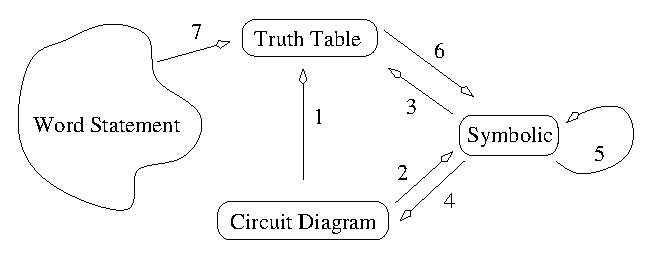
\includegraphics{./Fig2/forms}
\vspace{0.2in}

\begin{tabular}[ht]{l|l|l}
			& Regular Algebra		& Boolean Algebra \\ \hline \hline
Performed First	& Parenthesis		& Parenthesis \\ \hline
			& Exponents			& Not  \\  \hline
			& multiplication/division & And \\  \hline
Performed Last	& addition/subtraction 	& Or \\
\end{tabular}

\vspace{0.2in}

\begin{tabular}[ht]{|c|c|c|}\hline
Axiom	&	Primary &	Dual	\\ \hline
1.	&	x+0=x	&	x*1=x	\\ \hline
2.	&	x+1=1	&	x*0=0	\\ \hline
3.	&	x+x=x	&	x*x=x	\\ \hline
4.	&	x''=x	&	     	\\ \hline
5.	&	x+x'=1	&	x*x'=0	\\ \hline
6.	&	x+y=y+x	&	x*y=y*x\\ \hline
7.	& x+(y+z)=(x+y)+z&x*(y*z)=(x*y)*z \\ \hline
8.	& x*(y+z)=x*y+x*z  & x+(y*z)=(x+y)*(x+z)  \\ \hline
9.	& (x+y)'=x'*y'  & (x*y)'=x'+y' \\ \hline
\end{tabular}


%%%%%%%%%%%%%%%%%%%%%%%%%%%%%%%%%%%%%%%%%%%%%%%%%%%%
%% Here are terms that the students define
%%%%%%%%%%%%%%%%%%%%%%%%%%%%%%%%%%%%%%%%%%%%%%%%%%%%
\subsection{Definitions}
\begin{description}
\item[Expansion Trick]
\item[Minterm Trick]
\item[Minterm]
\item[Maxterm]
\end{description}


%%%%%%%%%%%%%%%%%%%%%%%%%%%%%%%%%%%%%%%%%%%%%%%%%%%%
%% Here are the problems
%%%%%%%%%%%%%%%%%%%%%%%%%%%%%%%%%%%%%%%%%%%%%%%%%%%%
\subsection{Problems}
Here is a list of problems.

{\bf Circuit Diagram to Truth Table}

\begin{tabular}{ll}
	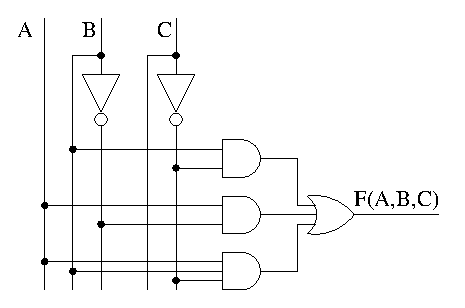
\includegraphics{./Fig2/cd-tt}
&
	\begin{tabular}{c|c|c||c}
	A & B & C & F(A,B,C) \\ \hline \hline
	0 & 0 & 0 &   \\ \hline
	0 & 0 & 1 &   \\ \hline
	0 & 1 & 0 &   \\ \hline
	0 & 1 & 1 &   \\ \hline
	1 & 0 & 0 &   \\ \hline
	1 & 0 & 1 &   \\ \hline
	1 & 1 & 0 &   \\ \hline
	1 & 1 & 1 &   \\
	\end{tabular}	\\
\end{tabular}

%% \item[Determine the symbolic for the circuit.]
%% \includegraphics{./FigWork/cd-sym-easy}

%% \item[Determine the symbolic for the circuit.]
%% \includegraphics{./FigWork/cd-sym-hard}


{\bf Symbolic to Circuit Diagram Easy}
\begin{tabular}{lp{2in}}
F(A,B,C)=AB'+A(B'+C)  & \\
\end{tabular}
\vspace{0.5in}

{\bf Symbolic to Circuit Diagram Hard}
\begin{tabular}{lp{2in}}
F(A,B,C,D)=A(BC+A(C'+D)')' + B'CD'  & \\
\end{tabular}
\vspace{0.5in}

\pagebreak
{\bf Symbolic to Truth Table Easy.}

\begin{tabular}{ll}
	F(A,B,C) = AB'+A(B'+C) & \\
	\begin{tabular}{c|c|c|c|c||c}
	A & B & C &   &    &  F(A,B,C) \\ \hline \hline
	0 & 0 & 0 &   &    &    \\ \hline
	0 & 0 & 1 &   &    &    \\ \hline
	0 & 1 & 0 &   &    &    \\ \hline
	0 & 1 & 1 &   &    &    \\ \hline
	1 & 0 & 0 &   &    &    \\ \hline
	1 & 0 & 1 &   &    &    \\ \hline
	1 & 1 & 0 &   &    &    \\ \hline
	1 & 1 & 1 &   &    &    \\
	\end{tabular} \\ 
\end{tabular}

\vspace{0.2in}

{\bf Symbolic to Truth Table Hard}

\begin{tabular}{ll}
	F(A,B,C,D)=A(BC+A(C'+D)')' + B'CD'  & \\
	\begin{tabular}{c|c|c|c||p{0.1in}|p{0.2in}|p{0.2in}|p{0.2in}|p{0.2in}||c}
	A & B & C & D &   &    &  &  &  & F(A,B,C,D) \\ \hline \hline
	0 & 0 & 0 & 0 &   &    &  &  &  &   \\ \hline
	0 & 0 & 0 & 1 &   &    &  &  &  &   \\ \hline
	0 & 0 & 1 & 0 &   &    &  &  &  &   \\ \hline
	0 & 0 & 1 & 1 &   &    &  &  &  &   \\ \hline
	0 & 1 & 0 & 0 &   &    &  &  &  &   \\ \hline
	0 & 1 & 0 & 1 &   &    &  &  &  &   \\ \hline
	0 & 1 & 1 & 0 &   &    &  &  &  &   \\ \hline
	0 & 1 & 1 & 1 &   &    &  &  &  &   \\ \hline
	1 & 0 & 0 & 0 &   &    &  &  &  &   \\ \hline
	1 & 0 & 0 & 1 &   &    &  &  &  &   \\ \hline
	1 & 0 & 1 & 0 &   &    &  &  &  &   \\ \hline
	1 & 0 & 1 & 1 &   &    &  &  &  &   \\ \hline
	1 & 1 & 0 & 0 &   &    &  &  &  &   \\ \hline
	1 & 1 & 0 & 1 &   &    &  &  &  &   \\ \hline
	1 & 1 & 1 & 0 &   &    &  &  &  &   \\ \hline
	1 & 1 & 1 & 1 &   &    &  &  &  &   \\ 
	\end{tabular} \\ 
\end{tabular}

\pagebreak

{\bf Truth Table to Symbolc}

\begin{tabular}{c|c|c||c|c|c}
A & B & C & F(A,B,C)	& minterm & maxterm	\\ \hline
0 & 0 & 0 & 0		&		& 	\\ \hline
0 & 0 & 1 & 1		& 		&	\\ \hline
0 & 1 & 0 & 1		& 		&	\\ \hline
0 & 1 & 1 & 1		& 		&	\\ \hline
1 & 0 & 0 & 1		& 		&	\\ \hline
1 & 0 & 1 & 0		& 		&	\\ \hline
1 & 1 & 0 & 0		& 		&	\\ \hline
1 & 1 & 1 & 1		& 		&	\\ 
\end{tabular}

\vspace{0.2in}

{\bf Word Statement to Truth Table}

Build 2 2-bit inputs A and B reprenting decimal numbers.  The single bit
output should equal 1 when A+B $>$ 6.
$$\begin{array}{c|c|c|c||c|c||c}
a_1 & a_0 & b_1 & b_0 & A  & B & F(a_1, a_0, b_1, b_0) 	\\ \hline
0 & 0 & 0 & 0 &  &  &   \\ \hline
0 & 0 & 0 & 1 &  &  &   \\ \hline
0 & 0 & 1 & 0 &  &  &   \\ \hline
0 & 0 & 1 & 1 &  &  &   \\ \hline
0 & 1 & 0 & 0 &  &  &   \\ \hline
0 & 1 & 0 & 1 &  &  &   \\ \hline
0 & 1 & 1 & 0 &  &  &   \\ \hline
0 & 1 & 1 & 1 &  &  &   \\ \hline
1 & 0 & 0 & 0 &  &  &   \\ \hline
1 & 0 & 0 & 1 &  &  &   \\ \hline
1 & 0 & 1 & 0 &  &  &   \\ \hline
1 & 0 & 1 & 1 &  &  &   \\ \hline
1 & 1 & 0 & 0 &  &  &   \\ \hline
1 & 1 & 0 & 1 &  &  &   \\ \hline
1 & 1 & 1 & 0 &  &  &   \\ \hline
1 & 1 & 1 & 1 &  &  &   \\ 
\end{array}$$


%% \index[Complete the timing diagraqm for the function $F(A,B,C) = A'B + AB'C$.]
%% 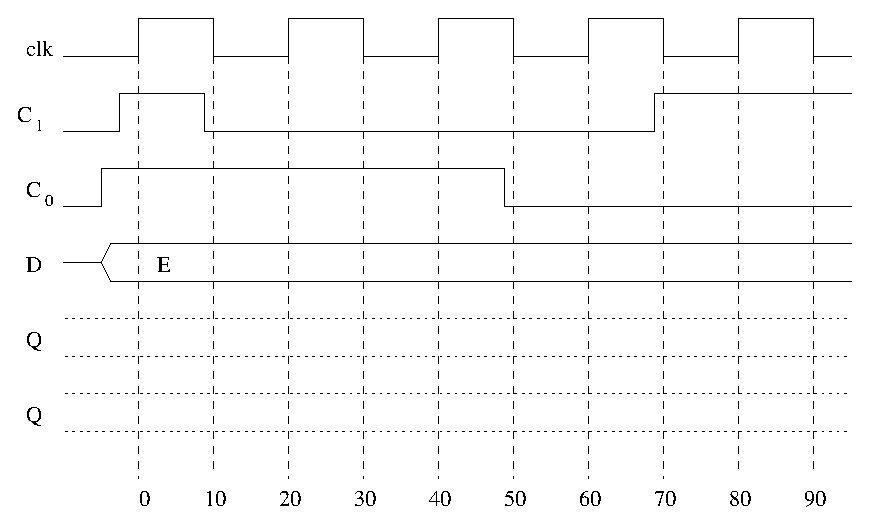
\includegraphics{./FigWork/time}
